%%
% !TeX program = xelatex
% !BIB program = biber
%%

\PassOptionsToClass{aspectratio=169}{ctexbeamer}
\documentclass[
  presentation,
  titlegraphic=./images/bit_logo.pdf,
  framelogo=./images/bit_logo.pdf
]{bitbeamer}

\title{IVOCT 钙化分割阶段性结果}
\author{CN\_seg 项目}
\institute{北京理工大学}
\date{2026-04-24}

\usefonttheme{serif}
\usefonttheme{professionalfonts}

\usepackage{graphicx}
\usepackage{caption}
\usepackage{subcaption}
\usepackage{booktabs}
\usepackage{array}
\usepackage{amsmath}
\usepackage{tikz}
\usepackage{xcolor}
\usepackage{multirow}
\usetikzlibrary{positioning}

\graphicspath{{figures/}}
\setbeamertemplate{caption}[numbered]
\setlength{\parskip}{0.25em}

\begin{document}

\frame{\titlepage}

\begin{frame}{汇报提纲}
  \tableofcontents[hideallsubsections]
\end{frame}

\AtBeginSection[]{\frame{\tableofcontents[currentsection,hideallsubsections]}}

\section{阶段目标}

\begin{frame}[t]{当前阶段目标}
  \begin{itemize}
    \item 基于已有 MAE 预训练 encoder，建立 IVOCT 钙化分割 baseline。
    \item 当前只有 4 名患者数据，重点是形成可复现的阶段性结果。
    \item 使用患者级 LOPO-CV 评估跨患者泛化能力。
    \item 等待剩余 14 名患者加入后，再重新判断是否需要改 loss、采样或模型结构。
  \end{itemize}

  \vspace{0.5cm}

  \begin{block}{当前主线结论}
    采用 \textbf{MAE encoder + Conv decoder} 的 reproduced baseline 作为当前正式 baseline；
    不继续围绕现有 4 名患者过度调参。
  \end{block}
\end{frame}

\begin{frame}[t]{数据与验证设计}
  \begin{columns}[T,onlytextwidth]
    \column{0.52\textwidth}
    \begin{table}
      \centering
      \small
      \begin{tabular}{cll}
        \toprule
        Fold & 训练患者 & 验证患者 \\
        \midrule
        0 & P002, P003, P004 & P001 \\
        1 & P001, P003, P004 & P002 \\
        2 & P001, P002, P004 & P003 \\
        3 & P001, P002, P003 & P004 \\
        \bottomrule
      \end{tabular}
    \end{table}

    \column{0.43\textwidth}
    \textbf{验证策略}
    \begin{itemize}
      \item Leave-One-Patient-Out
      \item 每折留出一名患者
      \item 更接近真实跨患者泛化评估
    \end{itemize}

    \vspace{0.25cm}

    \textbf{验证样本数}
    \begin{itemize}
      \item P001: 10 张
      \item P002: 14 张
      \item P003: 8 张
      \item P004: 11 张
    \end{itemize}
  \end{columns}
\end{frame}

\section{方法设置}

\begin{frame}[t]{模型与训练流程}
  \centering
  \begin{tikzpicture}[
    node distance=1.15cm,
    box/.style={draw, rounded corners=2pt, align=center, minimum width=2.8cm, minimum height=0.9cm},
    arrow/.style={->, thick}
  ]
    \node[box] (input) {IVOCT 图像\\$256\times256$};
    \node[box, right=of input] (mae) {MAE Encoder\\冻结};
    \node[box, right=of mae] (decoder) {Conv Decoder\\训练};
    \node[box, right=of decoder] (mask) {钙化区域\\分割预测};
    \draw[arrow] (input) -- (mae);
    \draw[arrow] (mae) -- (decoder);
    \draw[arrow] (decoder) -- (mask);
  \end{tikzpicture}

  \vspace{0.6cm}

  \begin{table}
    \centering
    \small
    \begin{tabular}{ll}
      \toprule
      项目 & 配置 \\
      \midrule
      Encoder & MAE pretrained encoder, frozen \\
      Decoder & Conv decoder \\
      ROI crop ratio & 0.86 \\
      Batch size & 4 \\
      Epochs & 300 \\
      Decoder learning rate & $1\times10^{-3}$ \\
      Weight decay & 0.05 \\
      Evaluation threshold & 0.3 \\
      \bottomrule
    \end{tabular}
  \end{table}
\end{frame}

\begin{frame}[t]{结果文件与可复现性}
  \begin{block}{服务器主线运行目录}
    \texttt{/root/CN\_seg\_baseline/seven/seg}
  \end{block}

  \begin{block}{主线结果文件}
    \texttt{/root/CN\_seg\_baseline/seven/seg/logs/results\_lopo\_20260424\_004401.json}
  \end{block}

  \begin{block}{本汇报包中保留的证据}
    \begin{itemize}
      \item \texttt{data/results\_lopo\_20260424\_004401.json}
      \item \texttt{data/checkpoint\_summary.json}
      \item \texttt{data/threshold\_sweep\_summary\_20260424\_baseline.json}
      \item \texttt{figures/fold\_*}
    \end{itemize}
  \end{block}
\end{frame}

\section{主线结果}

\begin{frame}[t]{LOPO-CV 主线结果}
  \begin{center}
    \Large
    \textbf{Mean Dice: $0.5212 \pm 0.1424$}
  \end{center}

  \vspace{0.25cm}

  \begin{table}
    \centering
    \small
    \begin{tabular}{ccccc}
      \toprule
      Fold & 验证患者 & Best Epoch & Dice Mean & IoU Mean \\
      \midrule
      0 & P001 & 177 & 0.5288 & 0.3746 \\
      1 & P002 & 168 & 0.2861 & 0.1805 \\
      2 & P003 & 52  & 0.6323 & 0.4643 \\
      3 & P004 & 94  & 0.6374 & 0.4775 \\
      \bottomrule
    \end{tabular}
  \end{table}

  \vspace{0.3cm}

  \begin{itemize}
    \item P003、P004 表现较好，P001 居中。
    \item P002 是当前最弱折，说明患者间泛化波动仍然明显。
  \end{itemize}
\end{frame}

\begin{frame}[t]{可视化结果：P001 与 P002}
  \begin{columns}[T,onlytextwidth]
    \column{0.49\textwidth}
    \centering
    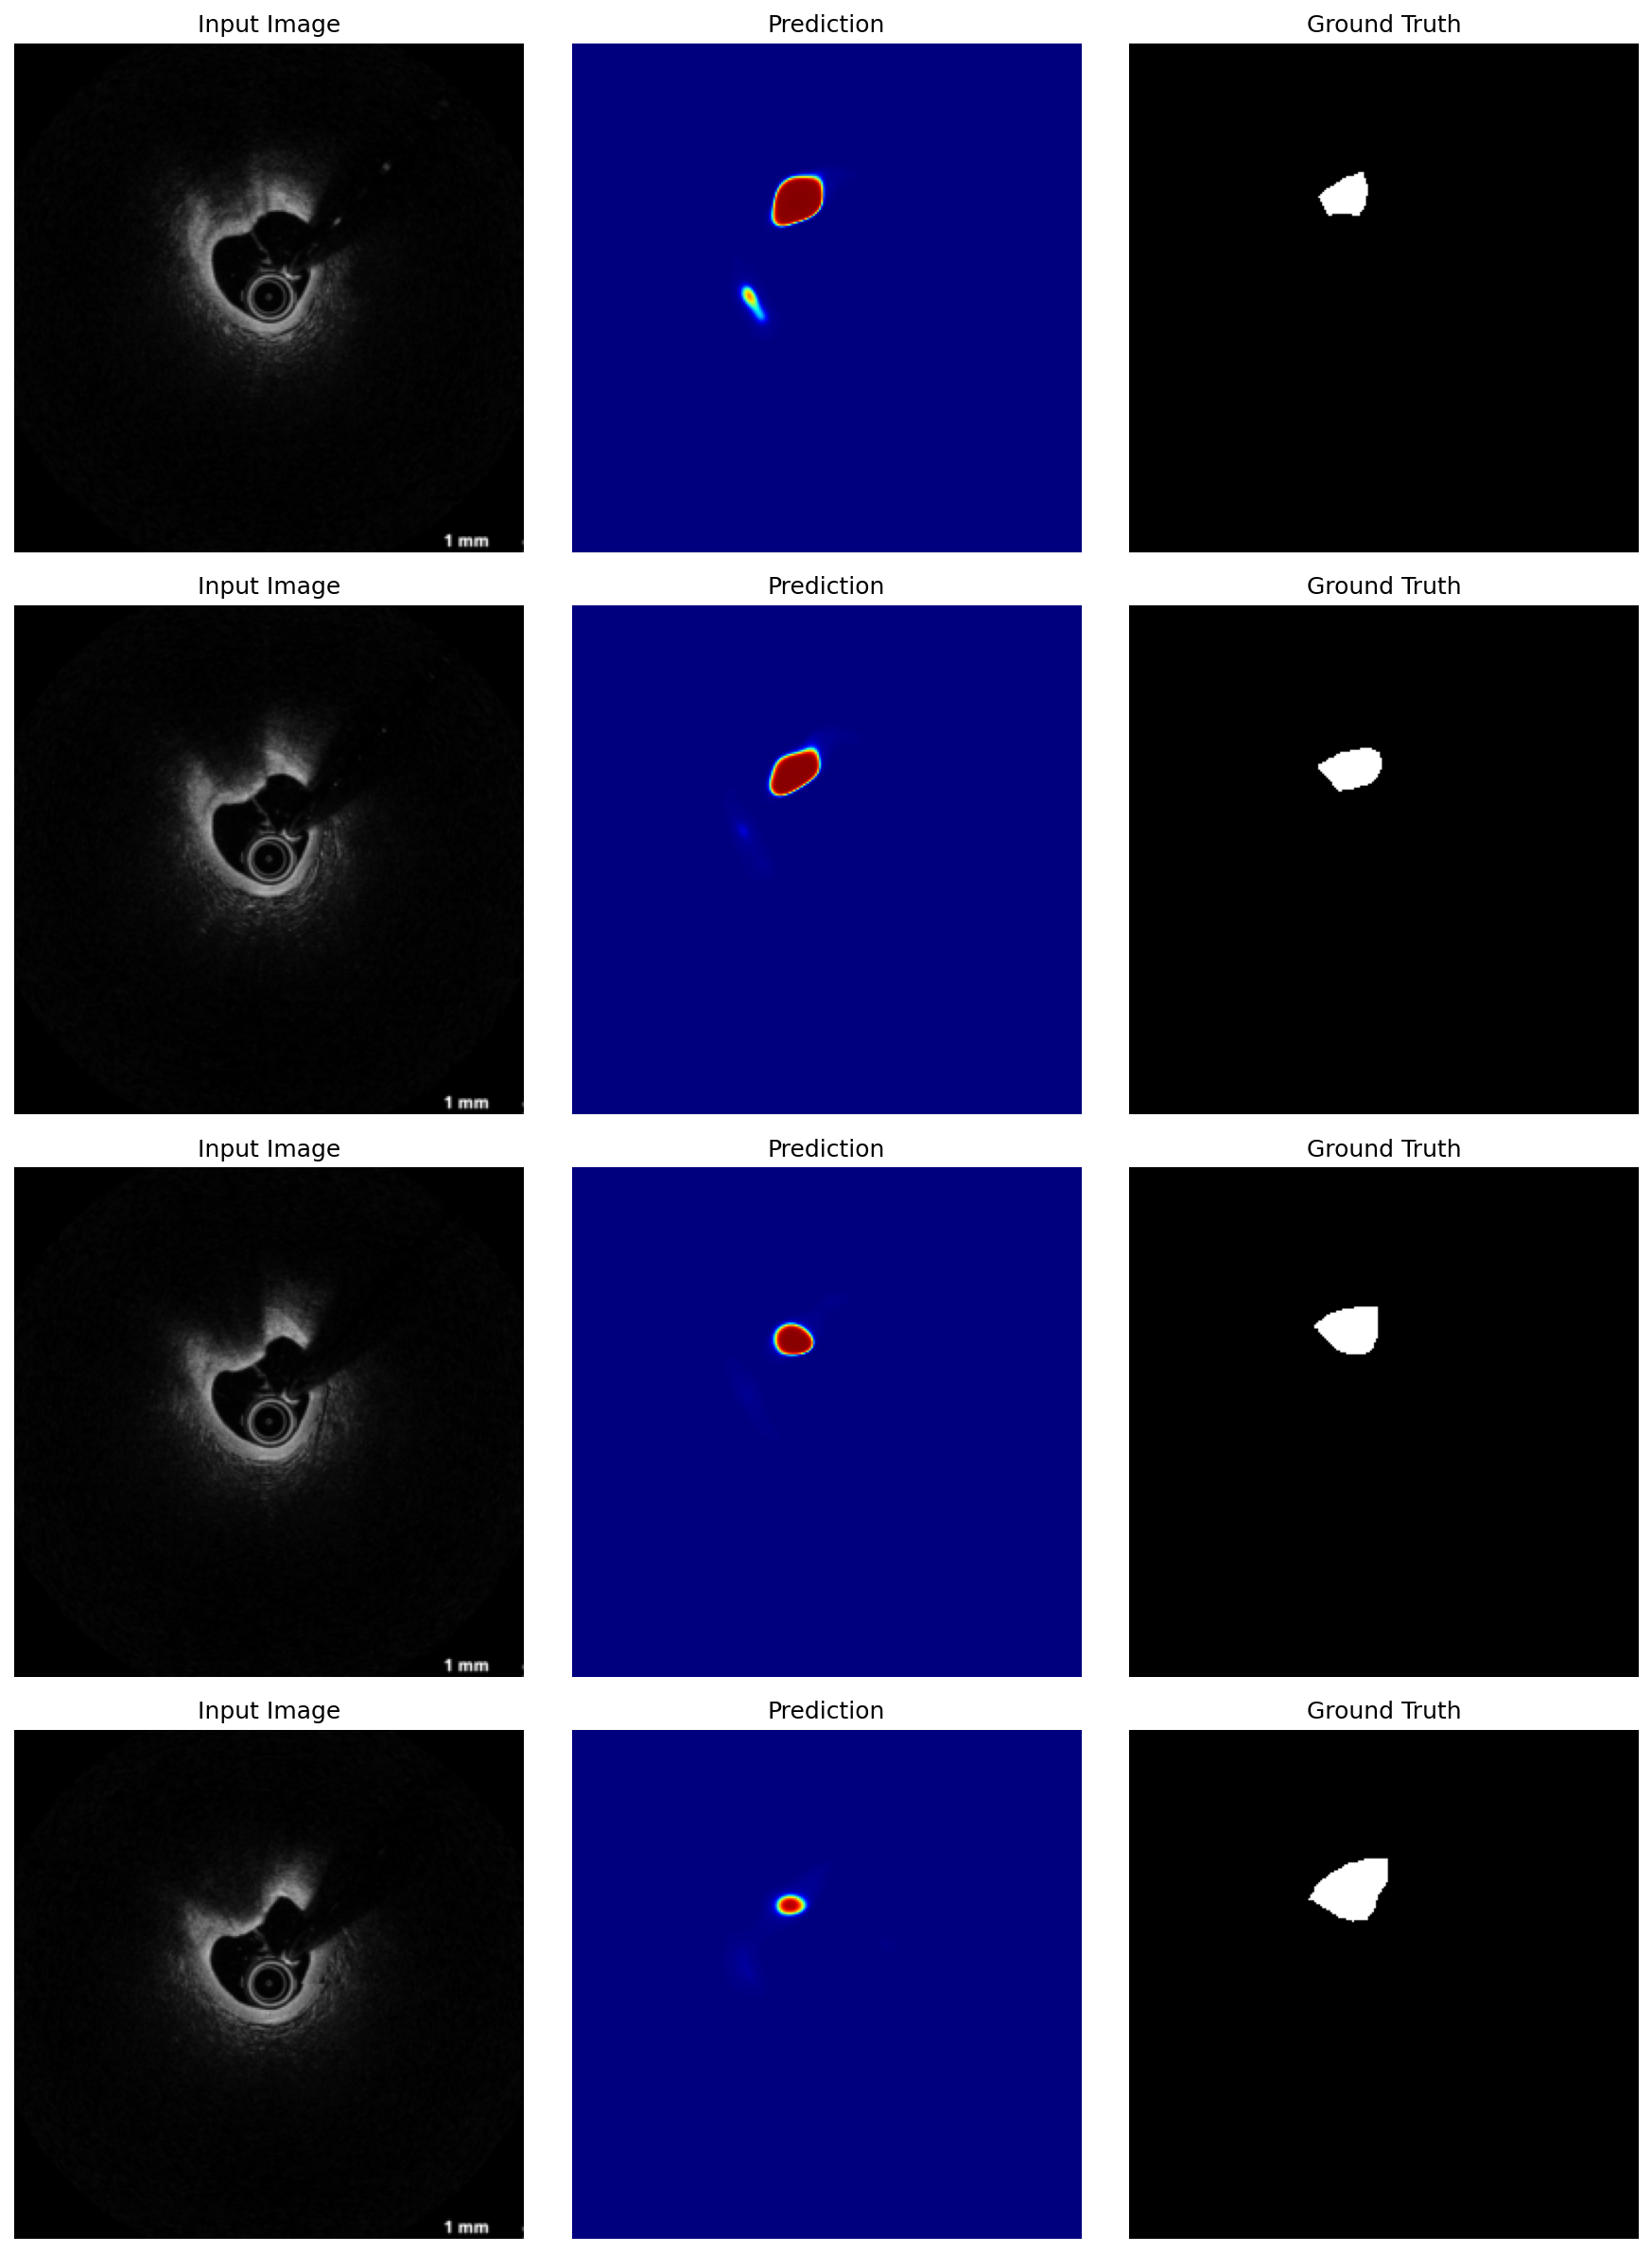
\includegraphics[width=\linewidth,height=0.68\textheight,keepaspectratio]{fold_0_best_epoch_177.png}
    \captionof{figure}{Fold 0, val=P001, Dice=0.5288}

    \column{0.49\textwidth}
    \centering
    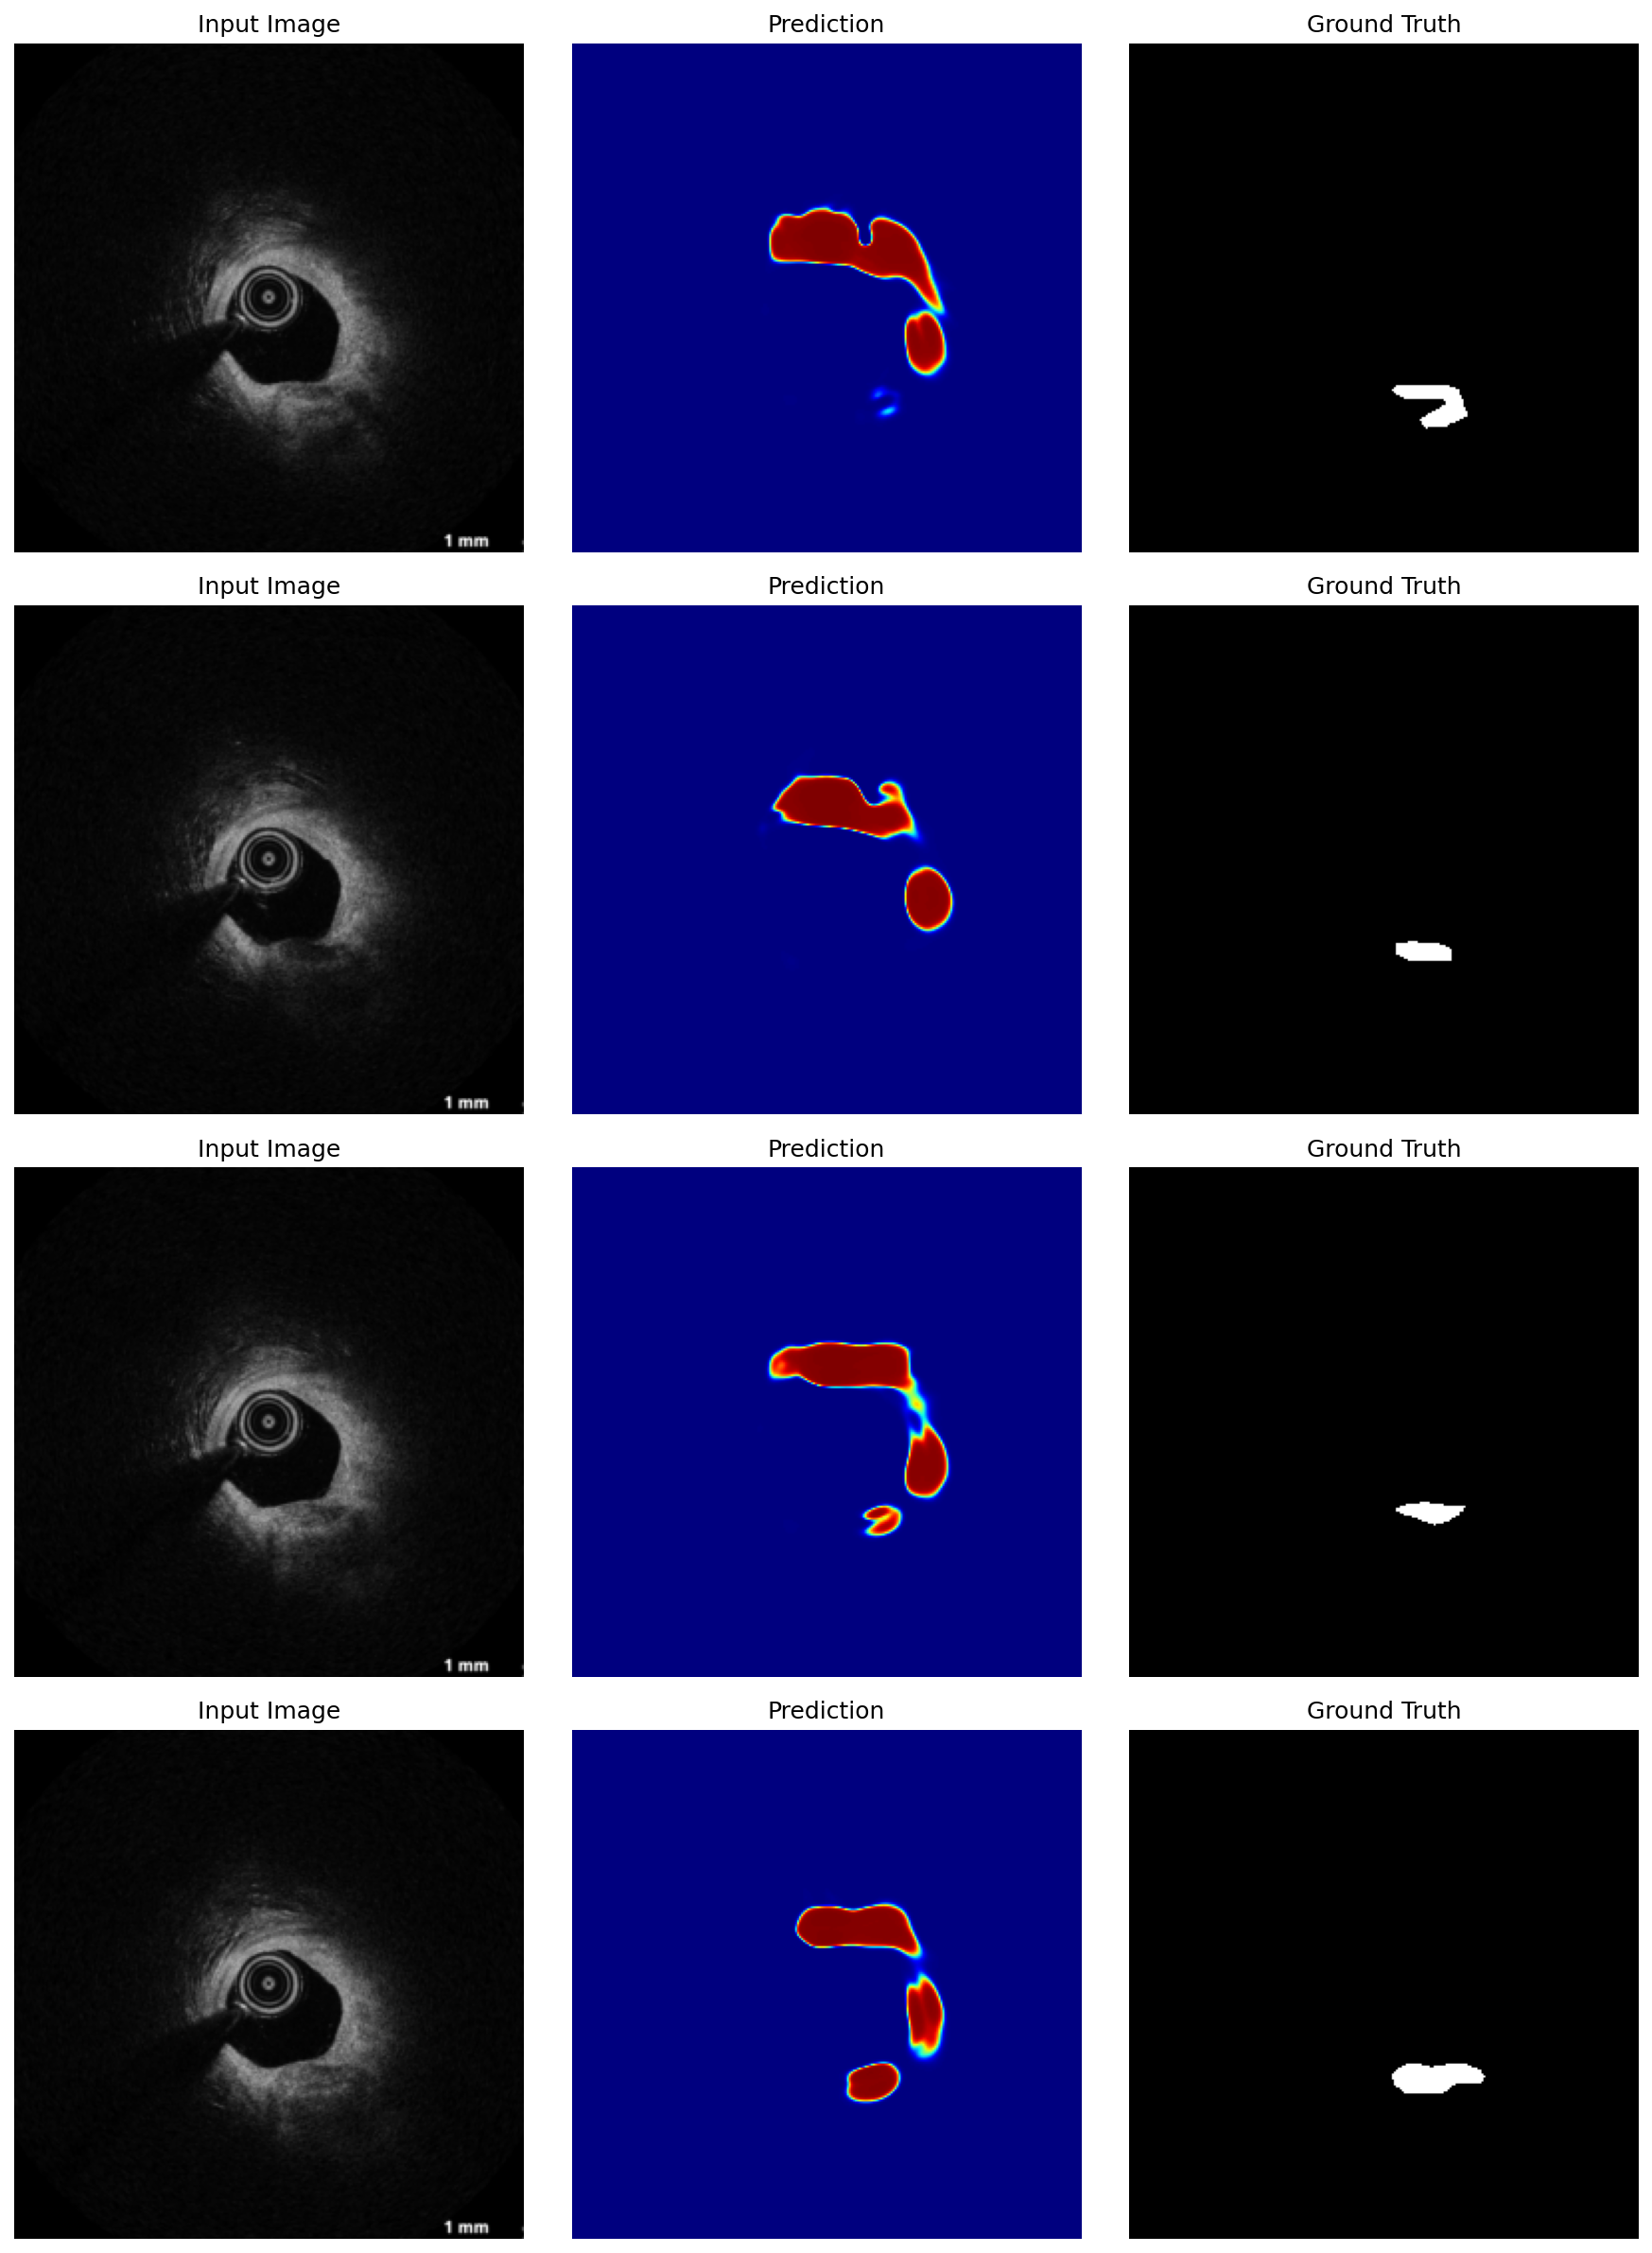
\includegraphics[width=\linewidth,height=0.68\textheight,keepaspectratio]{fold_1_best_epoch_168.png}
    \captionof{figure}{Fold 1, val=P002, Dice=0.2861}
  \end{columns}
\end{frame}

\begin{frame}[t]{可视化结果：P003 与 P004}
  \begin{columns}[T,onlytextwidth]
    \column{0.49\textwidth}
    \centering
    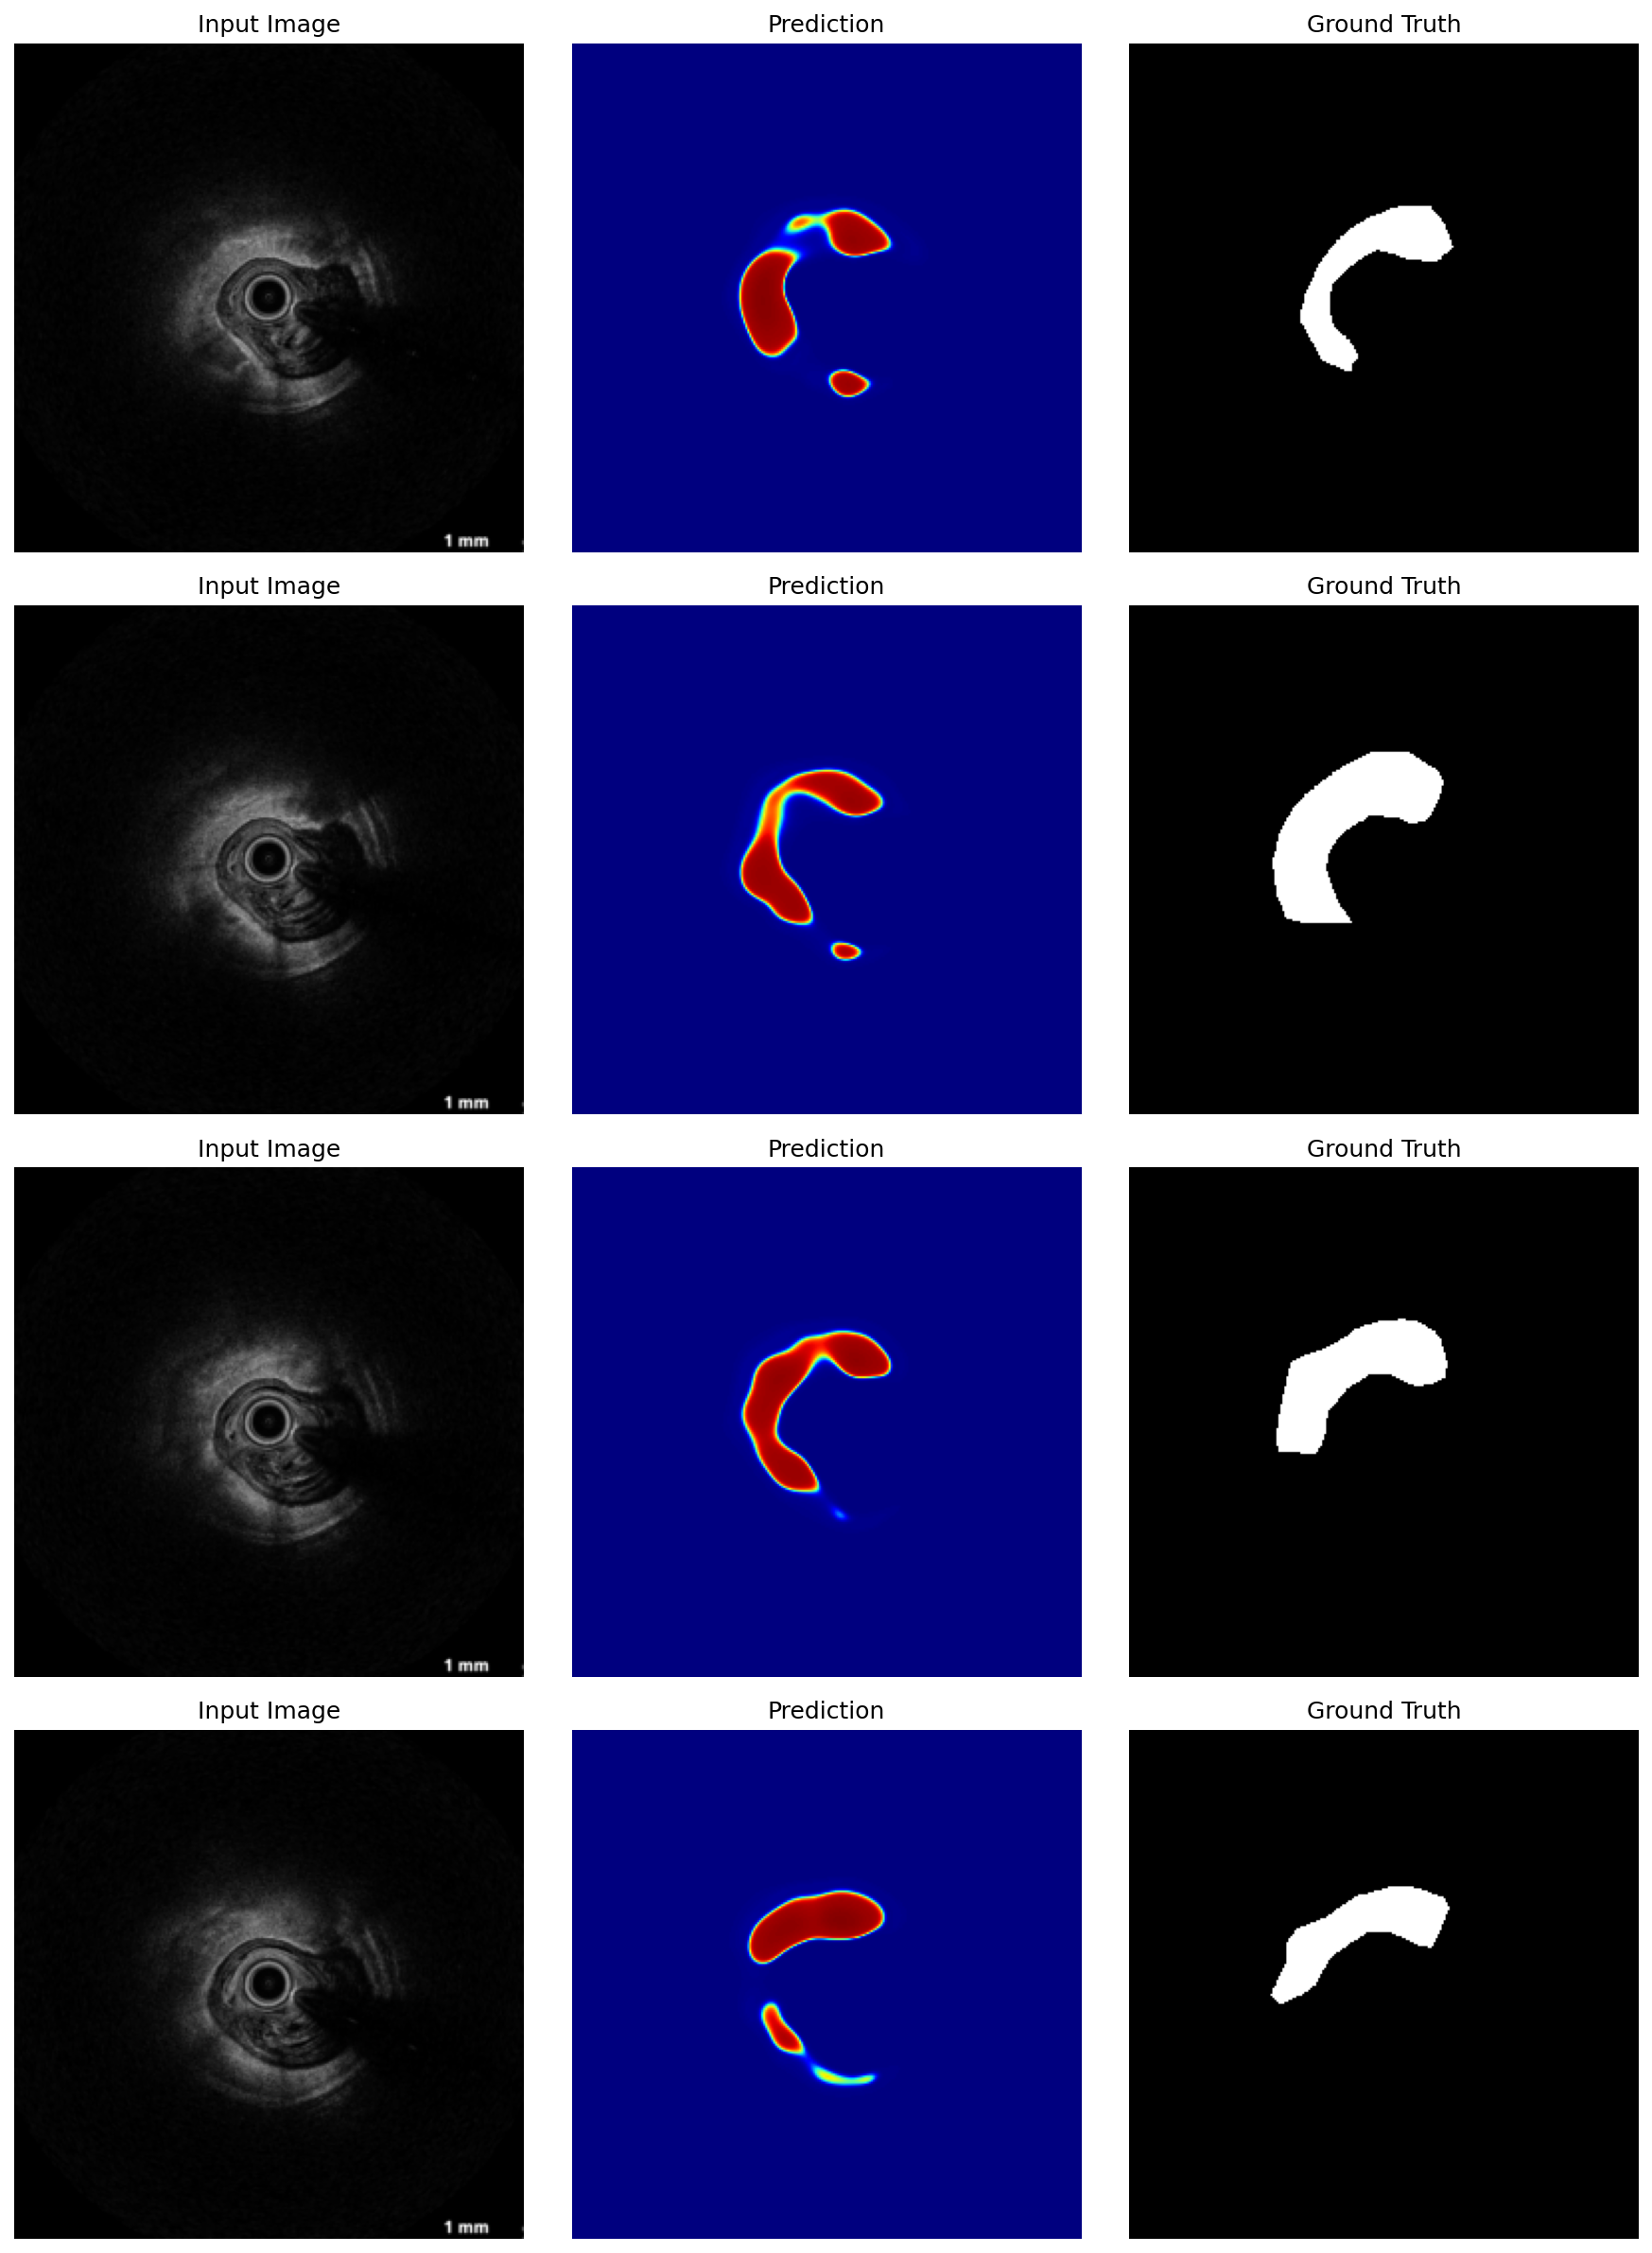
\includegraphics[width=\linewidth,height=0.68\textheight,keepaspectratio]{fold_2_best_epoch_052.png}
    \captionof{figure}{Fold 2, val=P003, Dice=0.6323}

    \column{0.49\textwidth}
    \centering
    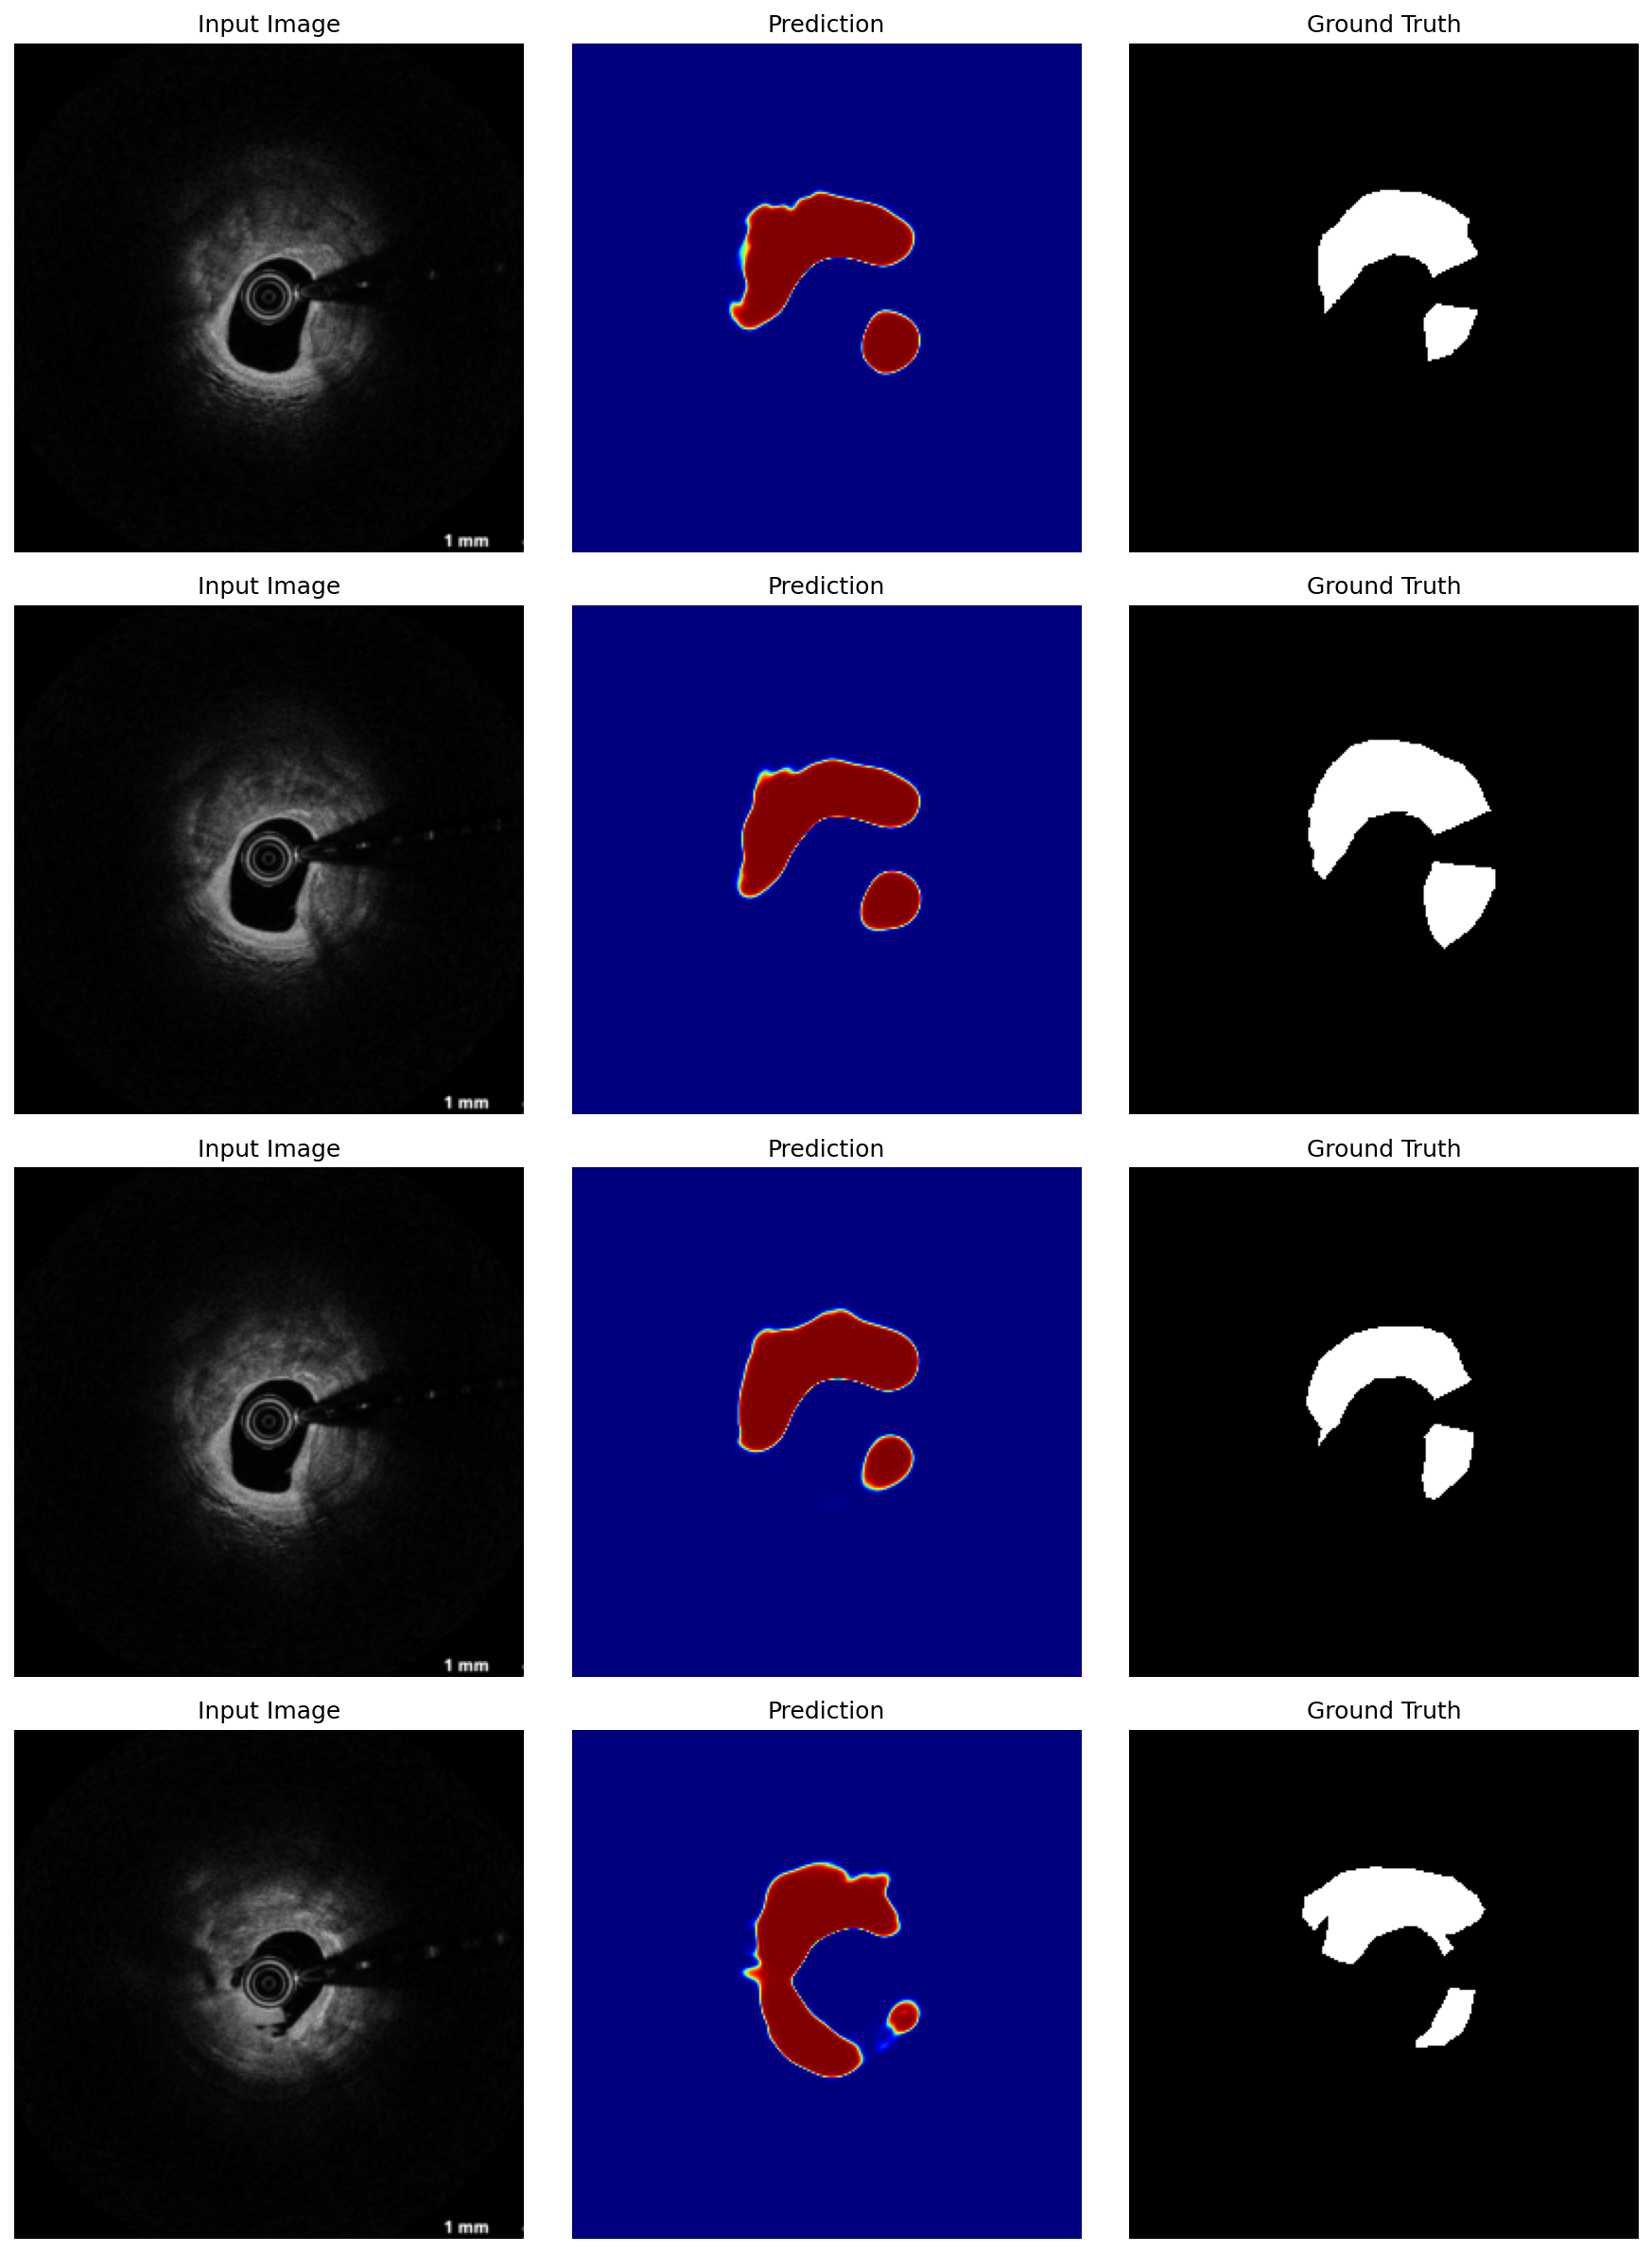
\includegraphics[width=\linewidth,height=0.68\textheight,keepaspectratio]{fold_3_best_epoch_094.png}
    \captionof{figure}{Fold 3, val=P004, Dice=0.6374}
  \end{columns}
\end{frame}

\section{补充分析}

\begin{frame}[t]{阈值扫描结论}
  \begin{columns}[T,onlytextwidth]
    \column{0.48\textwidth}
    \begin{table}
      \centering
      \small
      \begin{tabular}{cc}
        \toprule
        统一阈值 & Mean Dice \\
        \midrule
        0.3 & 0.5213 \\
        0.4 & 0.5169 \\
        0.5 & 0.5124 \\
        0.6 & 0.5091 \\
        0.7 & 0.5032 \\
        \bottomrule
      \end{tabular}
    \end{table}

    \column{0.48\textwidth}
    \begin{itemize}
      \item 全局统一最优阈值仍为 0.3。
      \item 阈值扫描没有带来实质全局提升。
      \item P002 单折最优阈值为 0.7，但 Dice 仅约 0.2895。
      \item P002 问题不是简单阈值校准，更像患者间泛化差异。
    \end{itemize}
  \end{columns}
\end{frame}

\begin{frame}[t]{已验证但未采用的方向}
  \begin{table}
    \centering
    \scriptsize
    \begin{tabular}{p{3.3cm}p{3.2cm}p{5.3cm}}
      \toprule
      方案 & 关键结果 & 判断 \\
      \midrule
      全局连通域后处理 & P002 提升，P003/P004 明显下降 & 不适合统一后处理 \\
      Focal alpha=0.5 & P002 Dice=0.2762 & 低于 baseline 的 0.2861 \\
      BN + early stopping & P002 Dice=0.2409 & 明显低于 baseline \\
      Focal Tversky + BN + early stopping & P002 LOPO Dice=0.3223，全局 Mean Dice=0.4561 & 改善 P002，但损害 P001/P003，全局不采用 \\
      \bottomrule
    \end{tabular}
  \end{table}

  \vspace{0.35cm}

  \begin{block}{阶段判断}
    当前样本量下，继续针对 P002 调整全局配置容易用整体性能换单折提升。
  \end{block}
\end{frame}

\section{阶段决策}

\begin{frame}[t]{当前阶段结论}
  \begin{enumerate}
    \item 当前正式 baseline：\textbf{MAE encoder + Conv decoder reproduced baseline}。
    \item 当前最优结果：Mean Dice $0.5212 \pm 0.1424$。
    \item 当前统一阈值：0.3。
    \item 当前主要问题：患者间泛化波动，尤其 P002 较弱。
    \item 当前策略：等待剩余 14 名患者加入后，再重新做 patient-level 泛化评估。
  \end{enumerate}

  \vspace{0.4cm}

  \begin{block}{建议}
    现阶段保留该 baseline 作为后续扩展数据实验的对照，不再围绕当前 4 名患者继续深度调参。
  \end{block}
\end{frame}

\begin{frame}[t]{下一步计划}
  \begin{itemize}
    \item 整合剩余 14 名患者数据，重新构建完整患者级评估集合。
    \item 继续使用当前 baseline 作为首个对照实验。
    \item 新数据加入后重新评估：
      \begin{itemize}
        \item LOPO-CV 的均值和方差；
        \item P002 型误差是否普遍存在；
        \item 是否需要引入采样策略、loss 调整或后处理。
      \end{itemize}
    \item 在更大样本规模下再决定是否进行结构性改动。
  \end{itemize}
\end{frame}

\begin{frame}[c]
  \centering
  \Huge 谢谢
\end{frame}

\end{document}
